\documentclass[compress,red]{beamer}
\usepackage[utf8]{inputenc}
\usepackage{ucs}
\usepackage{amsmath}
\usepackage{amsfonts}
\usepackage{amssymb}
\usepackage[russian]{babel}
\usepackage{graphicx}
\usepackage{wrapfig}

\usepackage{tikz}
\usepackage{verbatim}

\usepackage{color}
\usepackage{xcolor}
\usepackage{listings}

\usepackage{caption}
\DeclareCaptionFont{white}{\color{white}}
\DeclareCaptionFormat{listing}{\colorbox{gray}{\parbox{\textwidth}{#1#2#3}}}
\captionsetup[lstlisting]{format=listing,labelfont=white,textfont=white}

\usetikzlibrary{calc,trees,positioning,arrows,chains,shapes.geometric,%
    decorations.pathreplacing,decorations.pathmorphing,shapes,%
    matrix,shapes.symbols}

\tikzset{
>=stealth',
  punktchain/.style={
    rectangle, 
    rounded corners, 
    % fill=black!10,
    draw=black, very thick,
    text width=10em, 
    minimum height=3em, 
    text centered, 
    on chain},
  line/.style={draw, thick, <-},
  element/.style={
    tape,
    top color=white,
    bottom color=blue!50!black!60!,
    minimum width=8em,
    draw=blue!40!black!90, very thick,
    text width=10em, 
    minimum height=1.5em, 
    text centered, 
    on chain},
  every join/.style={->, thick,shorten <=1pt},
  decoration={brace},
  tuborg/.style={decorate},
  tubnode/.style={midway, right=2pt},
}

\mode<presentation>

\usetheme{Warsaw}

\definecolor{Red}{rgb}{1,0,0}
\definecolor{Blue}{rgb}{0,0,1}
\definecolor{Green}{rgb}{0,1,0}
\definecolor{magenta}{rgb}{1,0,.6}
\definecolor{lightblue}{rgb}{0,.5,1}
\definecolor{lightpurple}{rgb}{.6,.4,1}
\definecolor{gold}{rgb}{.6,.5,0}
\definecolor{orange}{rgb}{1,0.4,0}
\definecolor{hotpink}{rgb}{1,0,0.5}
\definecolor{newcolor2}{rgb}{.5,.3,.5}
\definecolor{newcolor}{rgb}{0,.3,1}
\definecolor{newcolor3}{rgb}{1,0,.35}
\definecolor{darkgreen1}{rgb}{0, .35, 0}
\definecolor{darkgreen}{rgb}{0, .6, 0}
\definecolor{darkred}{rgb}{.75,0,0}

\xdefinecolor{olive}{cmyk}{0.64,0,0.95,0.4}
\xdefinecolor{purpleish}{cmyk}{0.75,0.75,0,0}

\useoutertheme[subsection=false]{smoothbars}


\title{Основы программирования на ruby}
\author{Информатика \\ 10-11 классы}

%\usecolortheme{dolphin}


\begin{document}
%%титульная страница
\maketitle
%% основные моменты

\section{Введение}
\subsection{Как выучить C++ за 21 день?}
\begin{frame}
  \frametitle{Как выучить C++ за 21 день?}
	\centerline{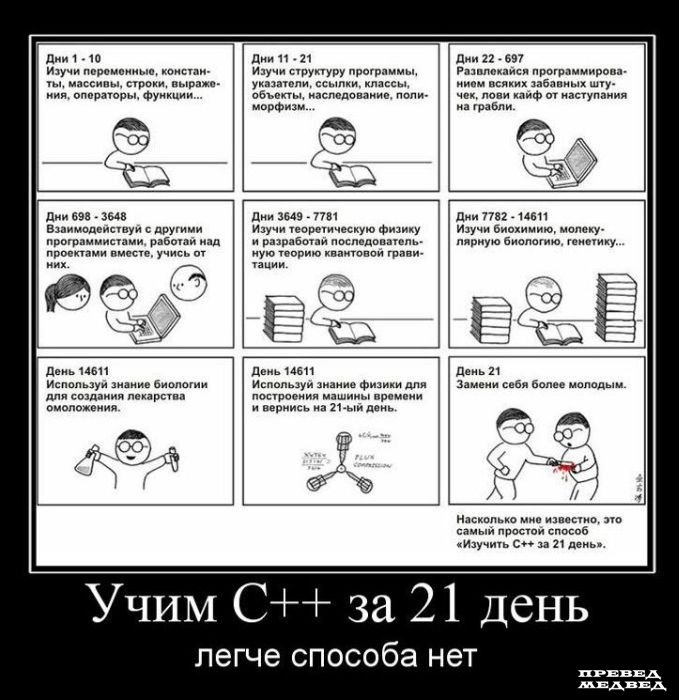
\includegraphics[width=0.6\textwidth]{images/how_to_learn_c.jpg}}
\end{frame}

\subsection{Что такое программирование?}
\begin{frame}
  \frametitle{Что такое программирование?}
  \begin{itemize}
	\item Программирование сродни переводу.
	\item Написать программу на языке программирования ничуть не сложнее, чем перевести фразу с русского на английский.
	\item Программа --- это последовательность команд, которые должен выполнить компьютер, чтобы получить нужный результат.
	\item Язык программирования, как и обычный язык, имеет свои \emph{лексические}, \emph{синтаксические} и \emph{семантические} правила.
	\end{itemize}
\end{frame}

\subsection{Создание программы}
\begin{frame}
\frametitle{Введение}
		
		\begin{figure}
    \centering
    \begin{tikzpicture}[node distance=1cm, auto]  
    \tikzset{
        mynode/.style={rectangle,rounded corners,draw=black, top color=white, bottom color=yellow!50,very thick, inner sep=0.7em, minimum size=1em, text centered},
        myarrow/.style={draw, thick, ->},
    }
    \node[mynode] (item1) {Идея};  
    \node[mynode, below=0.5cm of item1] (item2) {Алгоритм};
    \node[mynode, below=0.5cm of item2] (item3) {Блок--схема};
    \node[mynode, below=0.5cm of item3] (item4) {Программа};
    \node[mynode, below=0.5cm of item4] (item5) {:)};

    \draw[myarrow] (item1.south) -- (item2.north);   
    \draw[myarrow] (item2.south) -- (item3.north);   
    \draw[myarrow] (item3.south) -- (item4.north);   
    \draw[myarrow] (item4.south) -- (item5.north);   

    \end{tikzpicture} 
    \end{figure}
    
\end{frame}

\section{Основы программирования}
\subsection{Переменные}
\begin{frame}
  \frametitle{Переменные}
  \begin{itemize}
	\item Для работы программе нужно запоминать некоторые значения. Например, сайт ВКонтакте запоминает данные пользователя при входе в систему. 
	\item Такие значения называются \emph{переменные}.
	\item Переменные могут использоваться для различных целей. Например, в цикле считать количество проходов. Пример такой переменной: количество голов в футболе. На протяжении 90 минут эта переменная меняет своё значение в соответствии с ситуацией.
	\item Переменные бывают различных типов --- в зависимости от запоминаемых данных. Это --- строки, числа и пр.
	\end{itemize}
\end{frame}

\subsection{Типы переменных}
\begin{frame}
  \frametitle{Типы переменных}
  
  \begin{tabular}{|p{2cm}|p{2.5cm}|p{5.5cm}|}
  \hline
  Название & Перевод & Описание, примеры \\
  \hline
  integer & целое число & -1, 0, 1, 2, 500 ... \\
  \hline
  float & вещественное число & 1.05, $\pi$, $\sqrt{2}$ \\
  \hline
  string & строка & ``мама мыла раму'' \\
  \hline
  boolean & булевский & true (истина) / false (ложь), логический тип \\
  \hline
  array & массив & группа переменных [1,5,2] \\
  \hline
  hash & хэш & массив с текстовыми ключами \{~'name'~=>~'Вася',~'age'~=>~5~\} \\
  \hline
  object & объект &  \\
  \hline
  \end{tabular}
  
\end{frame}

\subsection{Integer \& Float: числа}
\begin{frame}
  \frametitle{Integer \& Float: числа}
	\begin{tabular}{|c|l|}
	\hline
	$+$ & сложение\\
	\hline
	$-$ & вычитание\\
	\hline
	$*$ & умножение\\
	\hline
	$/$ & (целочисленное) деление \\
	\hline
	$**$ & возведение в степень \\
	\hline
	$\%$ & остаток при делении\\
	\hline
	\end{tabular}
	
  \begin{itemize}
	\item $5 + 8*3 + 10 / 2 = 5 + 24 + 5 = 34 $
	\item $2**8 = 256$
	\item $14\%3 = 2$
	\item $15 / 4 = 3$ (целочисленное деление)
	\item $15.0 / 4 = 3.75$
	\end{itemize}
\end{frame}

\subsection{Строки и логические переменные}
\begin{frame}
  \frametitle{Строки и логические переменные}
  \begin{itemize}
    \item Контактация (сложение строк): ``мама'' + ``мыла раму'' = ``мамамыла раму''
    \item Обратите внимание! Пробел не добавляется, надо указывать вручную: ``мама ''
    \item Логические операции:
    \newline
    	\begin{tabular}{|c|c|c|}
    	\hline
    	$\&\&$ & конъюнкция & логическое ``и'' \\
    	\hline
    	$||$ & дизъюнкция & логическое ``или'' \\
    	\hline
    	$!$ & отрицание & логическое ``не'' \\
    	\hline
    	\end{tabular}
	\end{itemize}
\end{frame}

\section{Простейшие программы}
\subsection{Hello World!}
\begin{frame}[fragile]
  \frametitle{Hello World!}
  \begin{itemize}
    \item Первая программа, которую пишут начинающие программисты, --- Hello World. Программа делает единственную вещь: выводит на экран приветствие ``Hello world!''
    \item Напишем такую программу на языке программирования ruby.
  \end{itemize}
  \begin{lstlisting}[label=ruby1,caption=Hello World]
    puts "Hello world"
  \end{lstlisting}
  \begin{itemize}
    \item Оператор puts выводит любое сообщение или значение переменной на экран.
  \end{itemize}
\end{frame}

\subsection{Калькулятор}
\begin{frame}[fragile]
  \frametitle{Программа--Калькулятор}
  \begin{itemize}
    \item Сосчитаем следующие величины: $1024/13+523*2$, остаток от деления $2351$ на $37$, $2^{100}$, $2^{100}*50$
  \end{itemize}
  \begin{lstlisting}[label=ruby2,caption=Калькулятор]
    puts 1024.0/13+523*2
    puts 2351%37
    res = 2**100
    puts res
    puts res*50
  \end{lstlisting}
  \begin{itemize}
    \item Мы завели переменную res, чтобы сохранить результат $2^{100}$. Сохранив результат единожды, мы можем его использовать дальше в программе.
    \item Знак ``='' называется \emph{операцией присваивания}.
  \end{itemize}
\end{frame}

\subsection{Переменные}
\begin{frame}[fragile]
  \frametitle{Переменные}
  \begin{itemize}
    \item Переменные позволяют хранить промежуточные результаты вплоть до завершения программы.
    \item Переменных может быть сколько угодно (практически :) ).
    \item Допустим, есть две переменные $a$~и~$b$. Как их поменять местами, то есть сделать значение~$a$ равным~$b$, а $b$~---~$a$?
  \end{itemize}
  \begin{lstlisting}[label=ruby3,caption=Неправильный вариант]
    a = b
    b = a
  \end{lstlisting}
  \begin{itemize}
    \item Ошибка заключается в том, что компьютер выполняет команды последовательно.
    \item После выполнения команды $a~=~b$ обе переменные станут равными~$b$, а значение переменной~$a$ потеряется.
  \end{itemize}
\end{frame}

\subsection{Переменные}
\begin{frame}[fragile]
  \frametitle{Правильный вариант}
  \begin{itemize}
    \item Простой вариант не сработал, мы ``потеряли'' значение переменной~$a$.
    \item Логичное решение --- где-нибудь сохранить это значение. Но где?
    \item В другой переменной!
  \end{itemize}
  \begin{lstlisting}[label=ruby4,caption=Правильный вариант]
    c = a
    a = b
    b = c
  \end{lstlisting}
  \begin{itemize}
    \item Заметим, что в конце переменной~$b$ мы присваиваем значение переменной~$c$, так как~$a$~уже изменило своё значение и стала равной~$b$.
  \end{itemize}
\end{frame}

\section{Линейное уравнение}
\subsection{Линейное уравение}
\begin{frame}[fragile]
  \frametitle{Линейное уравнение}
  \begin{itemize}
    \item Рассмотрим чуть более сложную задачу: научим компьютер решать линейное уравнение $ax~+~b~=~c$. $a,b,c$ --- некоторые известные величины (параметры), а $x$ --- неизвестное, которое мы будем искать.
    \item Пример уравнения в числах: $2x~+~6 = 10$.
    \item Построение любой сложной программы прежде всего начинается с алгоритма.
    \item В нашем случае алгоритм прост:
      \begin{enumerate}
        \item Переносим b направо, чтобы все известные были справа, а неизвестные --- слева.
        \item Делим обе части равенства на $a$ (если $a \neq 0$).
        \item Получаем значение неизвестного $x$ и рассматриваем вариант $a = 0$.
      \end{enumerate}
    \item Следующим этапом является построение блок--схемы.
    \item Этот этап не всегда обязателен, но очень помогает начинающим не запутаться в сложных программах.
  \end{itemize}
\end{frame}

\subsection{Линейное уравнение}
\begin{frame}
  \frametitle{Блок--схема}
  \begin{figure}
  \centering
  \begin{tikzpicture}[node distance=1cm, auto]  
  \tikzset{
      action/.style={rectangle,draw=black, top color=white, bottom color=yellow!50,very thick, inner sep=0.25em, minimum size=0.6em, text centered},
      input/.style={ellipse,draw=black, top color=white, bottom color=yellow!50,very thick, inner sep=0.25em, minimum size=0.6em, text centered},
      condition/.style={diamond,draw=black, top color=white, bottom color=yellow!50,very thick, inner sep=0.25em, minimum size=0.6em, text centered},
      myarrow/.style={draw},
  }
  \node[input] (item1) {Ввести $a,b,c$};  
  \node[condition, below=1em of item1] (item2) {$a == 0$};
    \node[condition, right=of item2] (item3) {$b == c$};
      \node[action, below=of item3]  (item4) {Решений нет};
      \node[action, right=of item3] (item5) {$x$ --- любое};
    \node[action, left=of item2] (item6) {$x = (c-b)/a$};

  \path[myarrow] (item1) -- (item2);   
  \path[line] (item3) -- node [near end] {да} (item2);        
  \path[line] (item6) -- node [near end] {нет} (item2);        
  \path[line] (item4) -- node [near end] {нет} (item3);        
  \path[line] (item5) -- node [near end] {да} (item3);        

  \end{tikzpicture} 
  \end{figure}
\end{frame}

\end{document}